% Gráfico: Comparativo Geral - Gap de Otimalidade
\begin{figure}[htbp]
\centering
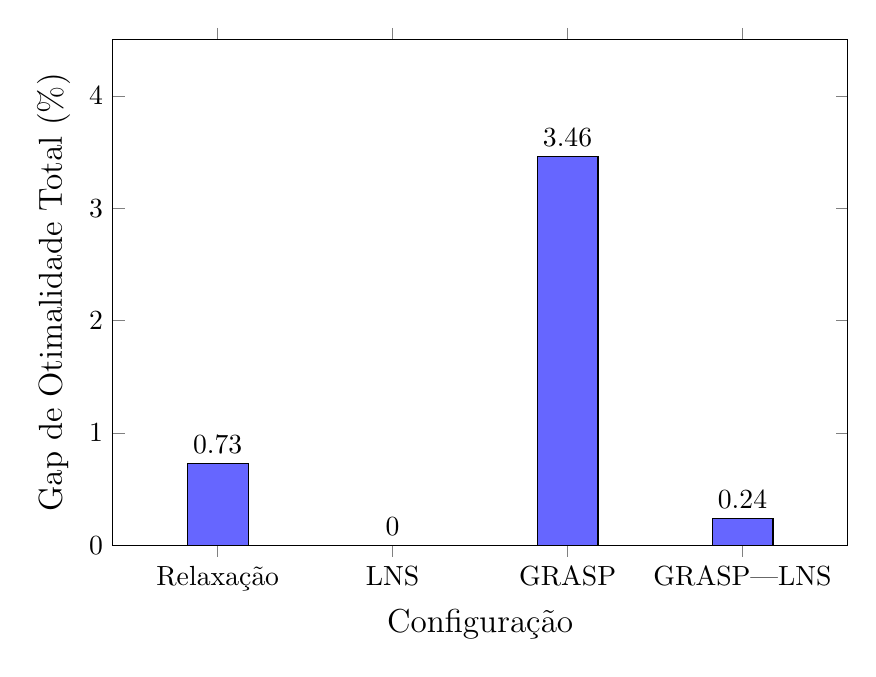
\begin{tikzpicture}
\begin{axis}[
    ybar,
    bar width=22pt,
    width=0.9\textwidth,
    height=8cm,
    ylabel={Gap de Otimalidade Total (\%)},
    xlabel={Configuração},
    symbolic x coords={Relaxação, LNS, GRASP, GRASP{|}LNS},
    xtick=data,
    nodes near coords,
    nodes near coords align={vertical},
    nodes near coords style={font=\normalsize, /pgf/number format/fixed,
        /pgf/number format/precision=2},
    ymin=0,
    ymax=4.5,
    enlarge x limits=0.2,
    ylabel style={font=\large},
    xlabel style={font=\large},
    tick label style={font=\normalsize},
]
\addplot[fill=blue!60] coordinates {
    (Relaxação,0.73)
    (LNS,0.00)
    (GRASP,3.46)
    (GRASP{|}LNS,0.24)
};
\end{axis}
\end{tikzpicture}
\caption{Gap de otimalidade total (\%) para cada configuração. O LNS atingiu gap zero, provando a otimalidade de todas as soluções encontradas.}
\label{fig:geral_gap}
\end{figure}
